This section covers some more fundamental theory on the topic of the thesis.
Mainly, it will cover the theory presented in many previous works.

A mathematician is a person who can calculate things~\parencite{wang2019cutting}.
That is good.
%
\begin{figure}[ht]
    \centering
    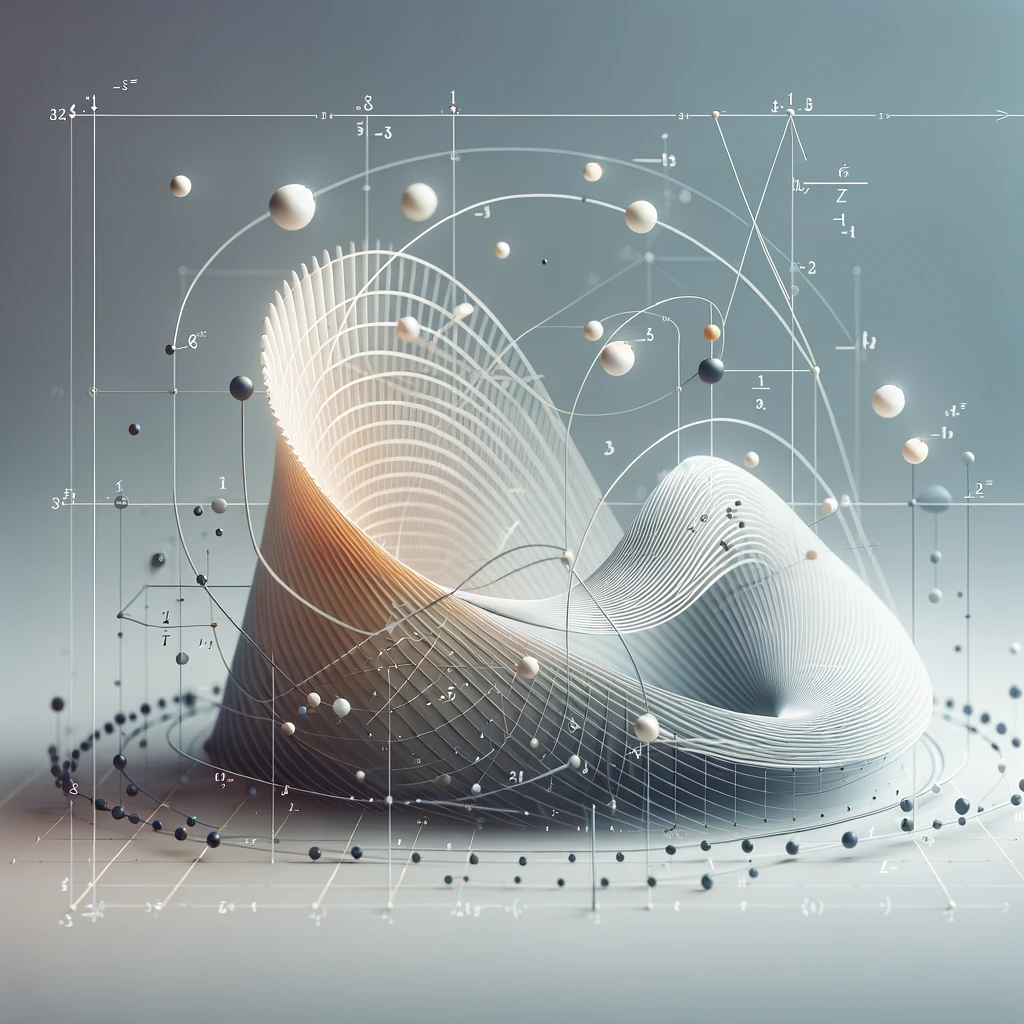
\includegraphics[width=0.3\textwidth]{src/figures/figure}
    \caption{Wow, look at this figure!}
    \label{fig:fun_figure}
\end{figure}
%
See Figure~\ref{fig:fun_figure} for a figure visualizing consequences of this fact.

In Algorithm~\ref{alg:universal_algorithm}, a very fun algorithm is presented.
%
\begin{algorithm}
    \caption{A very fun algorithm}
    \label{alg:universal_algorithm}
    \textbf{Let}
\begin{itemize}
	\item \(y\) be a symbol
	\item \(\epsilon_k\), \(k=1,\dots,K\), be a sequence of positive numbers
\end{itemize}

\textbf{Initialize} \(\hat{y}^{(0)} = \hat{y}\)
%
\[
	\hat{y} = \mathoperator{argmin}_{y \in \mathcal{Y}} \sum_{i=1}^n \mathcal{L}(y;\by_i)
\]
%

\textbf{For} \(k = 0,\dots,K-1\):
\begin{itemize}
	\item[] \textbf{For} \(\hat{A}_l \in \hat{A}^{(k)}\):
	\begin{enumerate}
		\item \textbf{Find}
		\[
			\hat{y}^{(k+1)} = \mathoperator{argmin}__{y \in \mathcal{Y}} \sum_{i=1}^n \mathcal{L}(y;\by_i)
			+ \sum_{i=1}^n \epsilon_k \mathcal{I}(y \neq \hat{y}^{(k)})
		\]
		\item \textbf{Stack}
		\[
			\hat{A}^{(k+1)} = \left[ \hat{A}^{(k)} \quad \hat{A}_l \right]
		\]
	\end{enumerate}

	\item[] \textbf{Return} \(\hat{y}^{(d_{\max})}\)
\end{itemize}

\end{algorithm}


